\chapter{العناصر في الكون وعلى الأرض}\label{ch:g9:elements-universe-earth}

الكالسيوم الذي في عظامك، والحديد الذي في دمك، والأكسجين الذي تتنفسه لم
تُصنع على الأرض. بل صُنعت في نجوم عاشت وماتت قبل أن تولد الشمس، وانتقلت
منذ مليارات السنين من الصخر إلى البحر، ومن البحر إلى النبات، ومن النبات إلى
الحيوان. بعض العناصر موجود في كل مكان، وبعضها نادر. فما العناصر التي تتكوّن
منها النجوم، والأرض، والمحيطات --- ونحن؟

\begin{recall}
\omterm{def:g9:inside-the-atom:element}{العنصر الكيميائي} مجموعة \omterm{def:g7:atoms-and-molecules:atom}{الذرات} التي لها \omterm{def:g9:inside-the-atom:atomic-number}{العدد الذري} $Z$ نفسه؛ وكتلة \omterm{def:g7:atoms-and-molecules:atom}{الذرة}
قريبة من $A \times \qty{1.67e-27}{kg}$، حيث $A$ عددها الكتلي
(\cref{ch:g9:inside-the-atom}). \omterm{def:g9:periodic-table-first-look:periodic-table}{والجدول الدوري} يذكر العناصر جميعها (118 عنصرًا) بحسب
عددها الذري (\cref{ch:g9:periodic-table-first-look}). \omterm{def:g4:air-a-mixture-of-gases:air}{والهواء} نحو أربعة
أخماسه نيتروجين وخمسه أكسجين (\cref{ch:g4:air-a-mixture-of-gases}).
\end{recall}

\section{عناصر النجوم}

\begin{definition}[الوفرة]\label{def:g9:elements-universe-earth:abundance}
\emph{وفرة}\index{وفرة} عنصر في جسم من المادة --- نجم، أو القشرة الأرضية،
أو المحيط، أو كائن حي --- هي نصيبه من الكتلة الكلية، وتُعطى عادة
بالنسبة المئوية.
\end{definition}

\begin{proposition}[الشمس هيدروجين وهيليوم]\label{prop:g9:elements-universe-earth:sun}
% ledger: ab:sun-X, ab:sun-Y, ab:sun-Z
سطح الشمس، بالكتلة، نحو \qty{74}{\percent} منه هيدروجين و\qty{25}{\percent}
هيليوم؛ أما سائر العناصر مجتمعة فلا تمثل إلا نحو \qty{1.3}{\percent}. ومعظم
المادة المرئية في الكون له تركيب مشابه: هيدروجين وهيليوم، مع رشّة من كل
ما عداهما.
\end{proposition}

\begin{proposition}[عناصر صُنعت في النجوم]\label{prop:g9:elements-universe-earth:stars}
تكوّن الهيدروجين ومعظم الهيليوم في الدقائق الأولى من عمر الكون. أما كل العناصر
الأثقل تقريبًا --- الكربون، والأكسجين، والحديد، والذهب --- فصُنعت لاحقًا،
داخل النجوم، وتناثرت في الفضاء حين انفجرت النجوم. ومن ذلك الغبار المُخصَّب
تكوّنت نجوم وكواكب جديدة. أما كيف تفعل النجوم ذلك فيرويه كتاب الفيزياء.
\end{proposition}

\begin{omfigure}
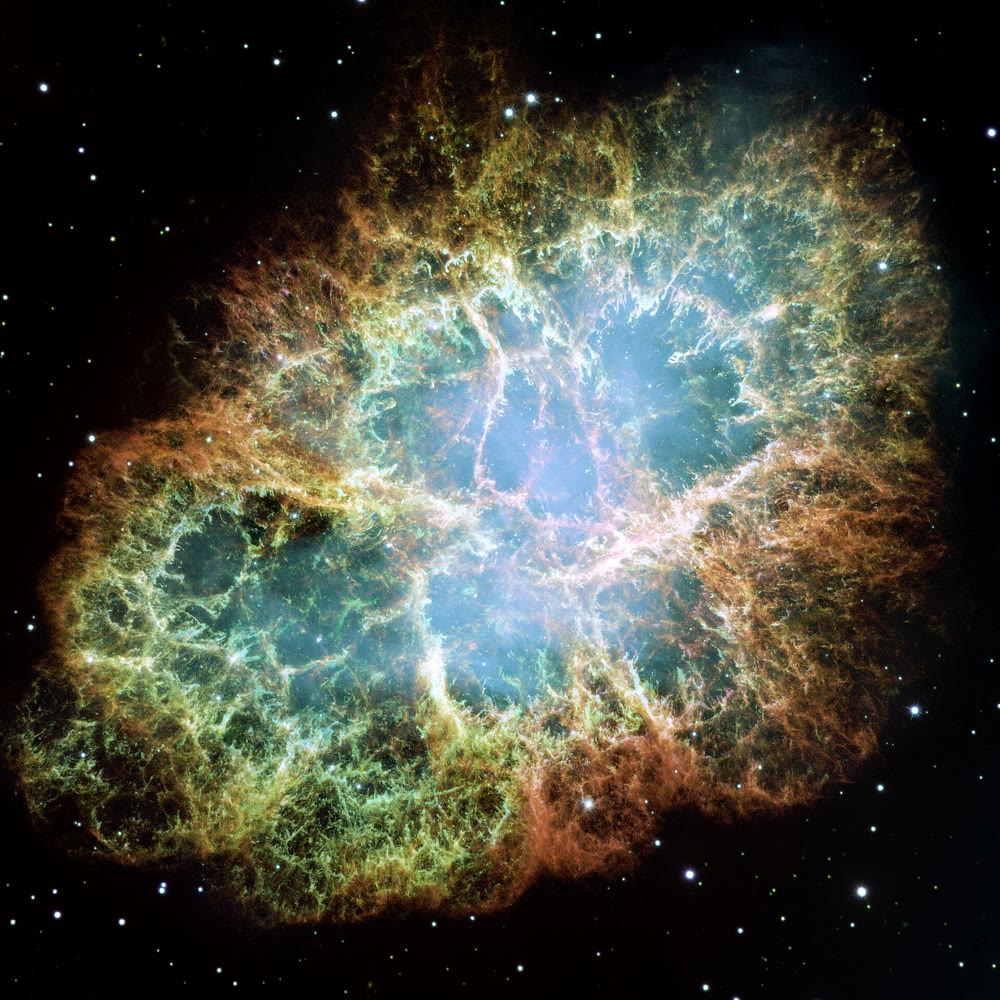
\includegraphics[width=0.45\linewidth]{images/book1/crab-nebula.jpg}

{\small سديم السرطان، السحابة التي خلّفها نجم انفجر قبل نحو ألف سنة، تنشر
عناصر جديدة في الفضاء (NASA وESA وج.~هستر
وأ.~لول).}
\end{omfigure}

\section{الأرض}

\begin{proposition}[القشرة الأرضية]\label{prop:g9:elements-universe-earth:crust}
% ledger: ab:crust-O, ab:crust-Si, ab:crust-Al, ab:crust-Fe, ab:crust-Ca, ab:crust-Na, ab:crust-K, ab:crust-Mg, ab:crust-first10
الغلاف الصخري الرقيق للأرض، أي القشرة، نصفه تقريبًا أكسجين وأكثر من ربعه
سيليكون بالكتلة: فالصخور والرمل في معظمها أكاسيد للسيليكون ولبضعة \omterm{def:g9:periodic-table-first-look:metal}{فلزات}.
وثمانية عناصر --- الأكسجين، والسيليكون، والألومنيوم، والحديد، والكالسيوم،
والصوديوم، والبوتاسيوم، والمغنيسيوم --- تمثل نحو \qty{99}{\percent} منها.
أما الهيدروجين والهيليوم، الشائعان جدًا في النجوم، فنادران: فقد أفلتت الغازات
الخفيفة من الأرض في شبابها.
\end{proposition}

\begin{remark}[داخل الأرض]\label{rem:g9:elements-universe-earth:core}
القشرة ليست الأرض كلها. فالحديد، لثقله، غاص نحو المركز حين كانت الأرض في
شبابها منصهرة: فلبّ الأرض في معظمه حديد، ومعه بعض
النيكل.
\end{remark}

\begin{proposition}[المحيطات والهواء]\label{prop:g9:elements-universe-earth:ocean}
% ledger: sea:salts-share, sea:NaCl-ions, sea:MgSO4-ions, air:N2, air:O2
ماء البحر في معظمه ماء --- هيدروجين وأكسجين --- ومعه نحو
\qty{3.5}{\percent} من الأملاح الذائبة بالكتلة. ومن بين \omterm{def:g9:ions:ion}{الأيونات} الذائبة
يمثل الكلوريد والصوديوم نحو \qty{85}{\percent}، والمغنيسيوم والكبريتات
\qty{10}{\percent} أخرى. \omterm{def:g4:air-a-mixture-of-gases:air}{والهواء} في معظمه نيتروجين
وأكسجين.
\end{proposition}

\begin{omfigure}
\begin{tikzpicture}
\begin{axis}[xbar, width=0.40\linewidth, height=5.4cm, xmin=0, xmax=85,
    bar width=7pt, symbolic y coords={Mg,K,Na,Ca,Fe,Al,Si,O}, ytick=data,
    xlabel={النسبة المئوية من الكتلة}, title={\small القشرة الأرضية},
    nodes near coords, nodes near coords style={font=\scriptsize},
    tick label style={font=\small}, label style={font=\small},
    axis lines*=left, enlarge y limits=0.08]
% ledger: ab:crust-O, ab:crust-Si, ab:crust-Al, ab:crust-Fe, ab:crust-Ca, ab:crust-Na, ab:crust-K, ab:crust-Mg
\addplot[fill=omDef!45, draw=omDef] coordinates {(46.6,O) (27.7,Si) (8.1,Al)
  (5.0,Fe) (3.6,Ca) (2.8,Na) (2.6,K) (2.1,Mg)};
\end{axis}
\end{tikzpicture}\hfill
\begin{tikzpicture}
\begin{axis}[xbar, width=0.40\linewidth, height=5.4cm, xmin=0, xmax=85,
    bar width=7pt, symbolic y coords={{P},{N},{Ca},{H},{C},{O}}, ytick=data,
    xlabel={النسبة المئوية من الكتلة}, title={\small جسم إنسان},
    nodes near coords, nodes near coords style={font=\scriptsize},
    tick label style={font=\small}, label style={font=\small},
    axis lines*=left, enlarge y limits=0.1]
% ledger: body:atoms-O, body:atoms-C, body:atoms-H, body:atoms-N, body:atoms-Ca, body:atoms-P (masses = atoms x atomic mass, over 70 kg)
\addplot[fill=omProp!45, draw=omProp] coordinates {(61.1,O) (22.9,C) (10.1,H)
  (1.3,N) (1.5,Ca) (0.7,P)};
\end{axis}
\end{tikzpicture}

{\small الوفرات بالكتلة. يمينًا: العناصر الثمانية الرئيسية في القشرة
الأرضية. يسارًا: العناصر الستة الرئيسية في جسم إنسان بالغ نحيل (محسوبة من
أعداد تقديرية \omterm{def:g7:atoms-and-molecules:atom}{للذرات}).}
\end{omfigure}

\section{جسم الإنسان}

\begin{proposition}[مِمَّ نتكون]\label{prop:g9:elements-universe-earth:body}
% ledger: body:atoms-O, body:atoms-C, body:atoms-H, body:atoms-N, body:atoms-Ca, body:atoms-P, body:atoms-total
بالكتلة، جسم البالغ النحيل نحو \qty{61}{\percent} منه أكسجين،
و\qty{23}{\percent} كربون، و\qty{10}{\percent} هيدروجين --- وهي في
معظمها في الماء وفي \omterm{def:g7:atoms-and-molecules:molecule}{جزيئات} الحياة --- يليها النيتروجين، والكالسيوم (في
العظام والأسنان)، والفوسفور. فإذا عُدّت \omterm{def:g7:atoms-and-molecules:atom}{الذرات} بدلًا من الكتلة تغيّر
الترتيب: ففي الجسم من \omterm{def:g7:atoms-and-molecules:atom}{ذرات} الهيدروجين أكثر من سائر \omterm{def:g7:atoms-and-molecules:atom}{الذرات} مجتمعة، لأن \omterm{def:g7:atoms-and-molecules:atom}{ذرات}
الهيدروجين بالغة الخفة. وجسم كتلته \qty{70}{kg} يحوي نحو
$7 \times 10^{27}$ \omterm{def:g7:atoms-and-molecules:atom}{ذرة}.
\end{proposition}

\begin{method}[قراءة مخطط الوفرة]\label{met:g9:elements-universe-earth:read}
\begin{enumerate}
  \item تحقق مما يُقاس: الكتلة (في معظم المخططات) أو عدد \omterm{def:g7:atoms-and-molecules:atom}{الذرات}.
  \item اقرأ نصيب كل عنصر؛ واجمع أنصبة الرئيسية منها لترى كم
        تغطي.
  \item لمقارنة جسمين، ابحث عن العناصر المشتركة بينهما وعن تلك التي
        لا توجد إلا في أحدهما.
\end{enumerate}
يتصدر الأكسجين مخططي هذا الفصل كليهما: فهو أشيع عناصر القشرة وعناصر جسم
الإنسان بالكتلة.
\end{method}

\section{الذرات نفسها، يُعاد تدويرها}

\begin{example}[رحلة ذرة كربون]\label{ex:g9:elements-universe-earth:journey}
\omterm{def:g7:atoms-and-molecules:atom}{ذرة} كربون صُنعت في نجم منذ زمن بعيد قد تبقى ملايين السنين في حجر جيري،
ثم يطلقها بركان على هيئة ثنائي أكسيد الكربون، فتأخذها ورقة نبات، وتصير جزءًا
من سكر في ثمرة، وتنتقل إلى حيوان يأكل الثمرة، ثم تُزفر من جديد على هيئة
ثنائي أكسيد الكربون. \omterm{def:g7:atoms-and-molecules:atom}{فالذرات} لا تفنى بالتغيرات الكيميائية: بل تنتقل من
مادة إلى أخرى.
\end{example}

\begin{omfigure}
\begin{tikzpicture}[font=\small,
    box/.style={draw=omDef, fill=omDef!6, rounded corners=2pt, align=center,
      minimum height=0.85cm, text width=2.3cm}]
  \node[box] (a) at (0,2.2) {في صخر\\ (حجر جيري)};
  \node[box] (b) at (4.3,2.2) {في الهواء\\ (\ce{CO2})};
  \node[box] (c) at (8.6,2.2) {في ورقة نبات\\ (سكر)};
  \node[box] (d) at (8.6,0) {في حيوان};
  \node[box] (e) at (4.3,0) {تُزفر\\ (\ce{CO2})};
  \draw[->, thick, omProp] (a) -- node[above, font=\footnotesize] {بركان} (b);
  \draw[->, thick, omProp] (b) -- (c);
  \draw[->, thick, omProp] (c) -- node[right, font=\footnotesize] {يأكلها} (d);
  \draw[->, thick, omProp] (d) -- (e);
  \draw[->, thick, omProp] (e) -- (b);
\end{tikzpicture}

{\small تنتقل \omterm{def:g7:atoms-and-molecules:atom}{ذرة} الكربون من الصخر إلى \omterm{def:g4:air-a-mixture-of-gases:air}{الهواء} إلى ورقة النبات إلى الحيوان ثم
تعود إلى \omterm{def:g4:air-a-mixture-of-gases:air}{الهواء}: \omterm{def:g7:atoms-and-molecules:atom}{والذرة} نفسها لا تفنى أبدًا.}
\end{omfigure}

\begin{omfigure}
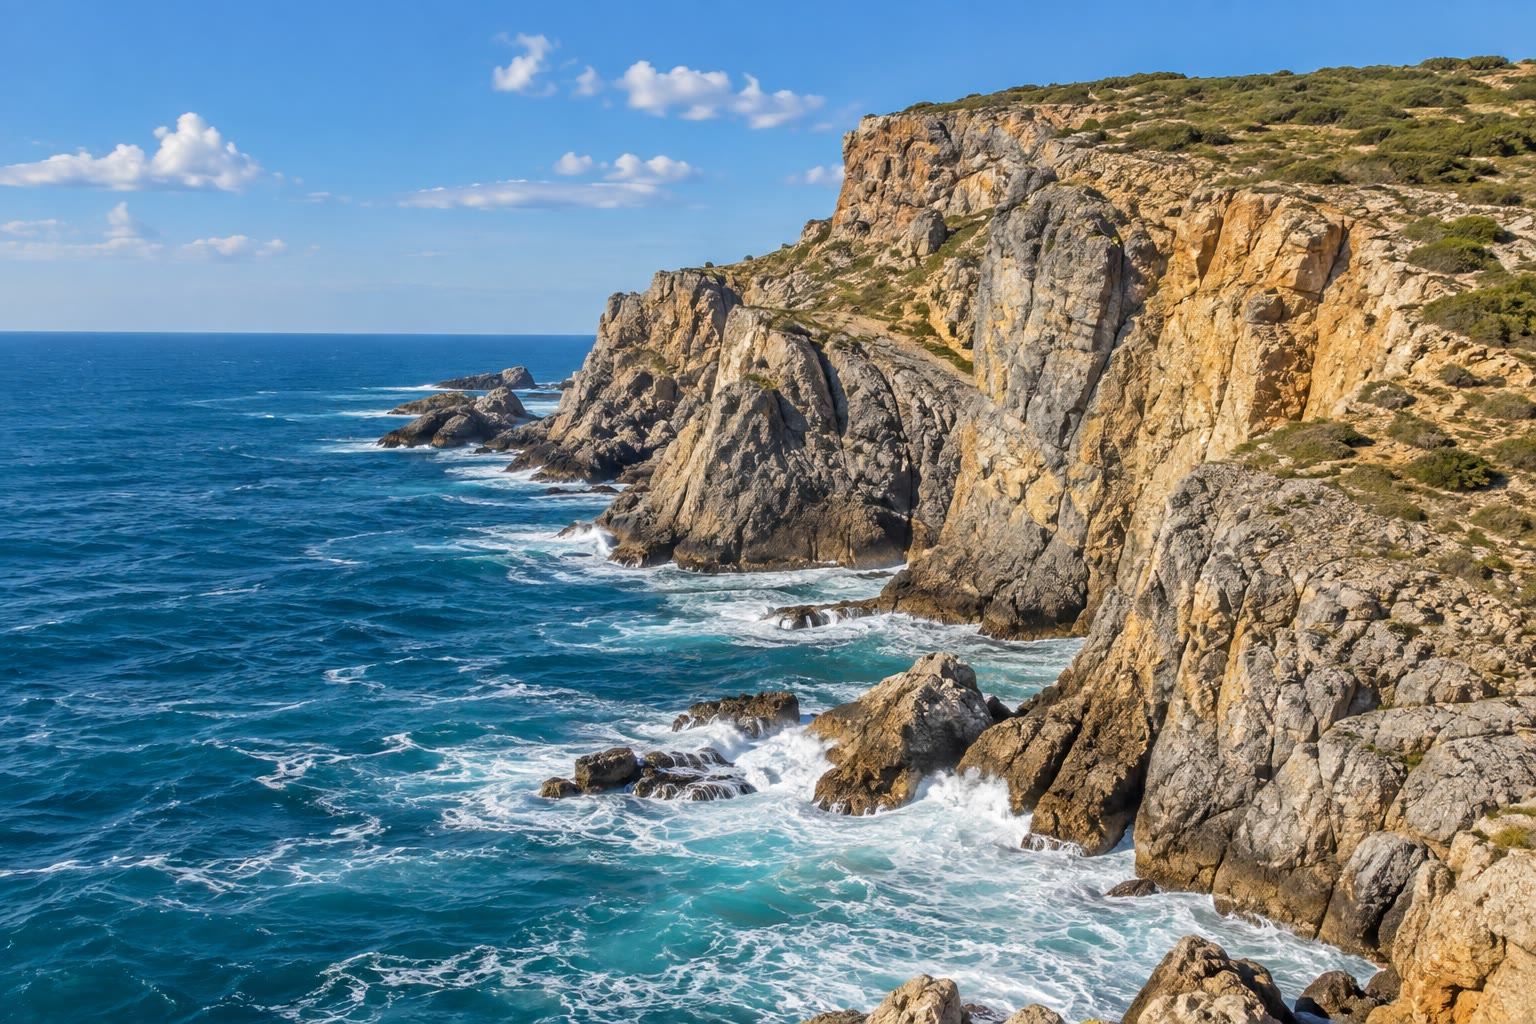
\includegraphics[width=0.55\linewidth]{images/book1/ai/g9-coastal-cliff.jpg}

{\small الصخر والبحر \omterm{def:g4:air-a-mixture-of-gases:air}{والهواء}: ثلاثة خلائط شديدة الاختلاف من العناصر
نفسها.}
\end{omfigure}

\section{تمارين}

\begin{exercise}[$\star$]\label{exo:g9:elements-universe-earth:1}
أي عنصرين يكوّنان الشمس كلها تقريبًا؟
\end{exercise}

\begin{exercise}[$\star$]\label{exo:g9:elements-universe-earth:2}
أي عنصر هو الأوفر في القشرة الأرضية؟ وفي جسم الإنسان
(بالكتلة)؟
\end{exercise}

\begin{exercise}[$\star$]\label{exo:g9:elements-universe-earth:3}
أين صُنعت معظم العناصر الأثقل من الهيليوم؟
\end{exercise}

\begin{exercise}[$\star$]\label{exo:g9:elements-universe-earth:4}
ما النسبة المئوية للملح الذائب من كتلة ماء البحر؟
\end{exercise}

\begin{exercise}[$\star\star$]\label{exo:g9:elements-universe-earth:5}
مستعينًا بمخطط القشرة، اجمع نصيبي الأكسجين والسيليكون. ما الكسر الذي
يمثله ذلك من القشرة تقريبًا؟
\end{exercise}

\begin{exercise}[$\star\star$]\label{exo:g9:elements-universe-earth:6}
لماذا يقل الهيدروجين والهيليوم كثيرًا في القشرة الأرضية، بينما تتكون
الشمس منهما كلها تقريبًا؟
\end{exercise}

\begin{exercise}[$\star\star$]\label{exo:g9:elements-universe-earth:7}
ما كتلة الكربون في جسم كتلته \qty{70}{kg} إذا كان
\qty{23}{\percent} منه كربونًا؟
\end{exercise}

\begin{exercise}[$\star\star$]\label{exo:g9:elements-universe-earth:8}
لماذا يكون الأكسجين أشيع عناصر الجسم بالكتلة، بينما يكون الهيدروجين
أشيعها بعدد \omterm{def:g7:atoms-and-molecules:atom}{الذرات}؟
\end{exercise}

\begin{exercise}[$\star\star$]\label{exo:g9:elements-universe-earth:9}
كتلة من الغرانيت وزنها \qty{1000}{kg} قطعة نموذجية من القشرة. مستعينًا
بالمخطط، ما كتلة الألومنيوم التي تحويها تقريبًا؟
\end{exercise}

\begin{exercise}[$\star\star$]\label{exo:g9:elements-universe-earth:10}
أي العناصر يظهر بين العناصر الرئيسية في القشرة وفي جسم الإنسان
كليهما؟
\end{exercise}

\begin{exercise}[$\star\star\star$]\label{exo:g9:elements-universe-earth:11}
جسم كتلته \qty{70}{kg} يحوي نحو \qty{1.06}{kg} من الكالسيوم. احسب
كتلة \omterm{def:g7:atoms-and-molecules:atom}{ذرة} كالسيوم واحدة ($A = 40$)، ثم عدد \omterm{def:g7:atoms-and-molecules:atom}{ذرات} الكالسيوم.
واكتبه بالكتابة العلمية.
\end{exercise}

\begin{exercise}[$\star\star\star$]\label{exo:g9:elements-universe-earth:12}
كانت \omterm{def:g7:atoms-and-molecules:atom}{ذرات} جسمك كلها جزءًا من أشياء أخرى من قبل. استعن برحلة \omterm{def:g7:atoms-and-molecules:atom}{ذرة}
الكربون لتشرح لماذا لا يكاد يتغير العدد الكلي \omterm{def:g7:atoms-and-molecules:atom}{لذرات} الكربون على
الأرض.
\end{exercise}

\section{مسألة: كم ذرة أنا؟}

\begin{problem}[{مسألة نهاية الأسبوع --- من مخطط الوفرة إلى عدد ذرات
الأكسجين في جسم الإنسان}]
\label{pb:g9:elements-universe-earth:1}
% ledger: body:atoms-O, body:atoms-total
بالغ نحيل كتلته \qty{70}{kg}، نحو \qty{61}{\percent} منه بالكتلة أكسجين،
و\qty{23}{\percent} كربون، و\qty{10}{\percent} هيدروجين. خذ
كتلة \omterm{def:g9:inside-the-atom:proton}{النوكليون} \qty{1.67e-27}{kg}؛ وفي \omterm{def:g7:atoms-and-molecules:atom}{ذرة} الأكسجين 16
نوكليونًا، وفي \omterm{def:g7:atoms-and-molecules:atom}{ذرة} الكربون 12، وفي \omterm{def:g7:atoms-and-molecules:atom}{ذرة} الهيدروجين 1. وتُهمل \omterm{def:g9:inside-the-atom:nucleus}{الإلكترونات}.

\medskip
\noindent\textbf{الجزء الأول --- الكتل.}
\begin{enumerate}
  \item احسب كتلة الأكسجين في الجسم.
  \item احسب كتلة الكربون وكتلة الهيدروجين.
  \item ما النسبة المئوية من الكتلة التي تمثلها هذه العناصر الثلاثة
        مجتمعة؟
  \item معظم هذا الأكسجين والهيدروجين في مركب واحد. ما هو؟
\end{enumerate}

\medskip
\noindent\textbf{الجزء الثاني --- \omterm{def:g7:atoms-and-molecules:atom}{ذرة} واحدة.}
\begin{enumerate}[resume]
  \item احسب كتلة \omterm{def:g7:atoms-and-molecules:atom}{ذرة} أكسجين واحدة.
  \item احسب كتلة \omterm{def:g7:atoms-and-molecules:atom}{ذرة} كربون واحدة وكتلة \omterm{def:g7:atoms-and-molecules:atom}{ذرة} هيدروجين واحدة.
  \item كم \omterm{def:g7:atoms-and-molecules:atom}{ذرة} هيدروجين تزن ما تزنه \omterm{def:g7:atoms-and-molecules:atom}{ذرة} أكسجين واحدة؟
  \item لماذا يجوز إهمال \omterm{def:g9:inside-the-atom:nucleus}{الإلكترونات}؟
\end{enumerate}

\medskip
\noindent\textbf{الجزء الثالث --- العدّ.}
\begin{enumerate}[resume]
  \item احسب عدد \omterm{def:g7:atoms-and-molecules:atom}{ذرات} الهيدروجين في الجسم.
  \item احسب عدد \omterm{def:g7:atoms-and-molecules:atom}{ذرات} الكربون.
  \item احسب عدد \omterm{def:g7:atoms-and-molecules:atom}{ذرات} الأكسجين في الجسم.
  \item يعطي تقدير دقيق $1.61 \times 10^{27}$ \omterm{def:g7:atoms-and-molecules:atom}{ذرة} أكسجين في مثل هذا
        الجسم. قارنه بحسابك، واذكر عدد \omterm{def:g7:atoms-and-molecules:atom}{ذرات} الأكسجين في جسم كتلته
        \qty{70}{kg} برقمين معنويين.
\end{enumerate}
\end{problem}
